\chapter{Ход работы}

\textbf{Цель работы}: провести модельное исследование параметрического параллельного стабилизатора при использовании стабилитрона \textbf{BZT52C15}.

Исходные данные: условия (дано) из ДЗ и результаты расчетов

\begin{figure}[h!]
	\centering
	\caption{Схема параметрического параллельного стабилизатора}
	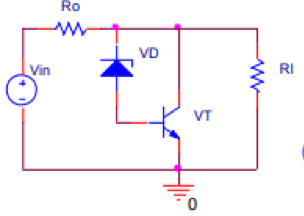
\includegraphics{images/scheme1.png}
\end{figure}


\begin{figure}[h!]
	\centering
	\caption{Модель системы в OrCAD Capture}
	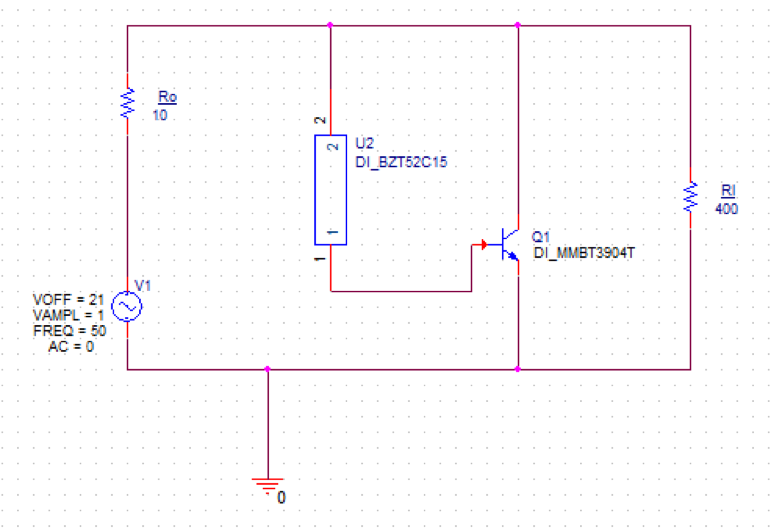
\includegraphics{images/scheme2.png}
\end{figure}

\section{Результаты моделирования}

\begin{figure}[h!]
	\centering
	\caption{Входное напряжение (зеленый, В), выходное напряжение (синий, В)}
	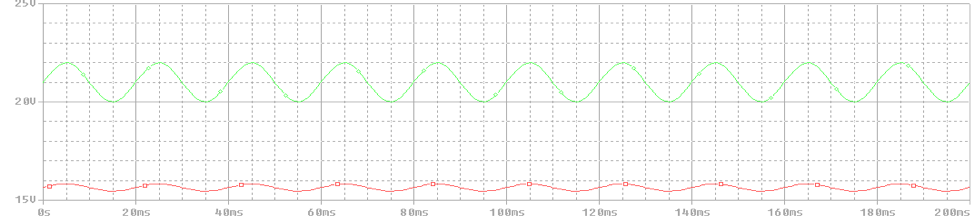
\includegraphics{images/model1.png}
\end{figure}

\begin{figure}[h!]
	\centering
	\caption{Напряжение на нагрузке (красный, А), среднее напряжение на нагрузке (зеленый, А)}
	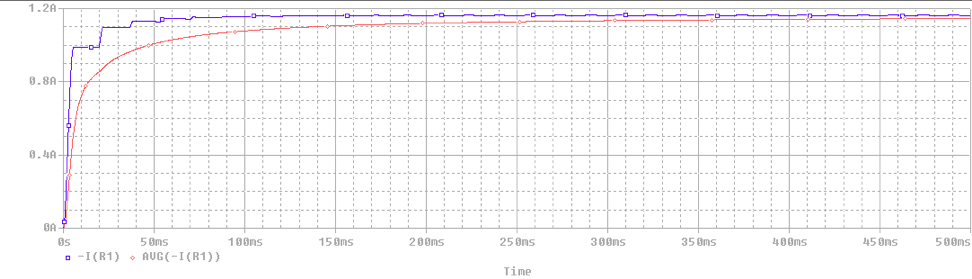
\includegraphics{images/model2.png}
\end{figure}

\begin{figure}[h!]
	\centering
	\caption{Ток на нагрузке (синий, А), средний ток на нагрузке (зеленый, А)}
	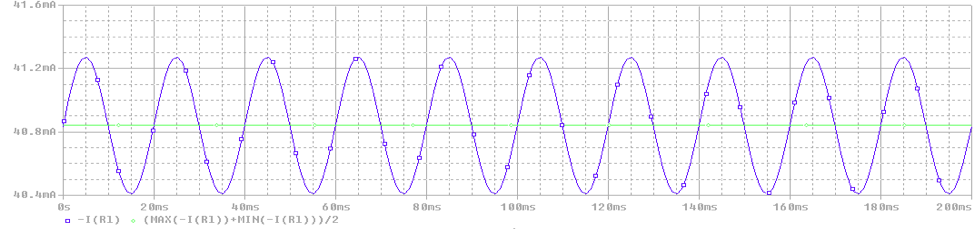
\includegraphics{images/model3.png}
\end{figure}

\begin{figure}[h!]
	\centering
	\caption{Ток через на балластном резисторе (синий, А), среднее значение тока (зеленый, А)}
	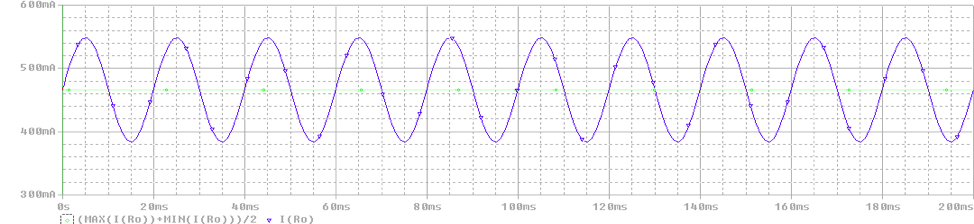
\includegraphics{images/model4.png}
\end{figure}


\section{Измерения в OrCAD Capture}

Выходное напряжение, В:

\[
U_{OUT\_EXP} = 15.644 
\]

Ток нагрузки, А:			        				

\[
I_{L\_EXP}=0.04081
\]

Средний ток на $R_O$, А:	         					

\[
I_{O\_EXP}=0.465
\]

Амплитуда пульсаций выходного напряжения, В:	

\[
\Delta U_{OUT\_EXP}=0.182
\]

Коэффициент стабилизации:				

\[
K_{ST\_EXP}=4.09
\]


\section{Вычисление погрешностей}

Погрешность $U_{OUT}$:

\[
\left|\frac{U_{OUT\_EXP}-U_{OUT}}{U_{OUT}} \right| = 4 \%
\]

Погрешность $I_L$:

\[
\left| \frac{I_{L\_EXP}-I_L}{I_L} \right|=9 \%
\]

Погрешность $I_O$: 

\[
\left| \frac{I_{O\_EXP}-I_O}{I_0} \right|= 6 \%
\]

Погрешность $\Delta U_{OUT}$:

\[
\left|  \frac{\Delta U_{OUT\_EXP}-\Delta U_{OUT}}{\Delta U_{OUT}} \right| =6 \%
\]

Погрешность $K_{ST}$:

\[
\left| \frac{K_{ST\_EXP}-K_{ST}}{K_{ST}} \right|=11\%
\]

\chapter{Вывод}

В ходе выполнения лабораторной работы было был промоделирован параллельный параметрический стабилизатор, построены графики изменения величин в OrCAD PSpice, измерены необходимые величины по этим графикам и рассчитаны погрешности.

Погрешность коэффициента стабилизации превышает 10\%, но
 превышение незнечительно, что свидетельствует о корректности выполнения работы и соответствии модели расчетным значениям.
